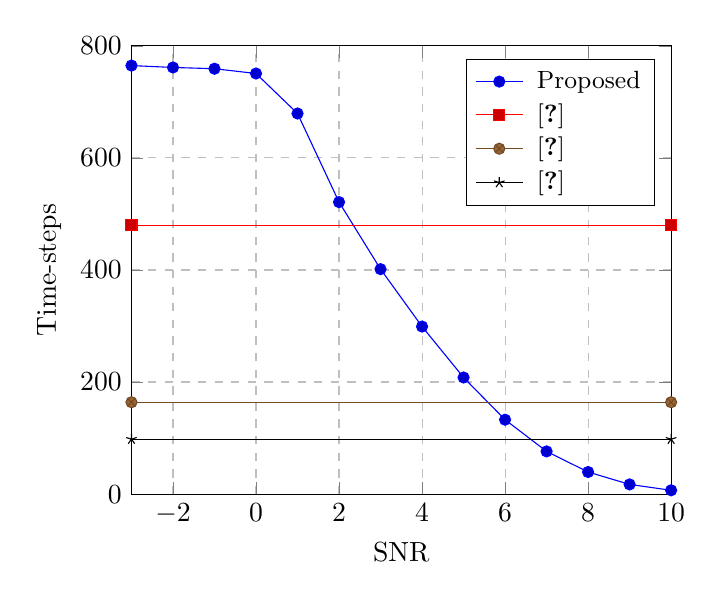
\begin{tikzpicture}

\begin{axis}[
scale=1,
xmin=-3,
xmax=10,
ymin=0,
ymax=800,
ymajorgrids=true,
xmajorgrids=true,
grid style=dashed,
%width=\textwidth, height=\textwidth,
xlabel={SNR},
ylabel={Time-steps},
%ylabel shift=-7,
legend cell align={left},
legend pos=north east,
legend style={
	column sep= 1mm,
	font=\fontsize{9pt}{9}\selectfont,
},
%legend to name=legend-BECcomp,
%legend columns=2,
]

%\addplot
%table {
%-3 96.74
%-2 95.27
%-1 91.81
%0 85.23
%1 75.11
%2 62.16
%3 48.16
%4 34.86
%5 23.24
%6 14.11
%7 7.77
%8 3.57
%9 1.37
%10 0.42
%};
%\addlegendentry{GA}

\addplot
table {
-3 764.73
-2 761.38
-1 759.11
0  750.57
1  679.21
2  521.09
3  401.47
4  299.03
5  208.15
6  132.79
7  76.27
8  39.48
9  17.33
10 6.86
};
\addlegendentry{Proposed}

\addplot
table {
-3 480
10 480
};
\addlegendentry{\cite{alamdar2011simplified}}

\addplot
table {
-3 164
10 164
};
\addlegendentry{\cite{sarkis2014fast}}

\addplot
table {
-3 98
10 98
};
\addlegendentry{\cite{hanif2017fast}}

\end{axis}
\end{tikzpicture}